\documentclass[aspectratio=169]{beamer}

\usetheme{Madrid}
\usecolortheme{default}
\setbeamertemplate{navigation symbols}{}
\setbeamertemplate{footline}[frame number]

\usepackage{booktabs}
\usepackage{graphicx}
\usepackage{amsmath}
\usepackage{xcolor}

\graphicspath{{../results/plots/}{../results/insights/}}

% Colour shortcuts
\newcommand{\good}[1]{\textcolor{green!60!black}{#1}}
\newcommand{\bad}[1]{\textcolor{red!70!black}{#1}}
\newcommand{\note}[1]{\textcolor{gray}{#1}}

% -------------------------------------------------------
\title[Cross-Language Vulnerability Detection]{%
  Cross-Language Software Vulnerability Detection\\
  via Fine-Tuned Pre-Trained Code Models}
\subtitle{Synthetic Training, Real-World Generalisation,\\and Semantic Understanding}
\author{[Author Name]}
\institute{University Dissertation}
\date{April 2026}
% -------------------------------------------------------

\begin{document}

% ===== TITLE =====
\begin{frame}
  \titlepage
\end{frame}

% ===== OUTLINE =====
\begin{frame}{Outline}
  \tableofcontents
\end{frame}

% =====================================================================
\section{Motivation}
% =====================================================================

\begin{frame}{The Problem: Polyglot Codebases}
  \begin{columns}
    \begin{column}{0.55\textwidth}
      \begin{itemize}
        \item $\sim$80\% of real projects use 7+ languages
        \item Vulnerability patterns differ \emph{per language}:
          \begin{itemize}
            \item Memory errors $\to$ C/C++
            \item Injection flaws $\to$ every language, different APIs
          \end{itemize}
        \item Existing tools are \textbf{monolingual}
          \begin{itemize}
            \item Flawfinder, Coverity: one language, hand-written rules
            \item Managing multiple tools $\to$ alert fatigue
          \end{itemize}
      \end{itemize}
    \end{column}
    \begin{column}{0.42\textwidth}
      \begin{block}{The gap}
        No single trained model that detects vulnerabilities
        across C \emph{and} Python, evaluated at the individual
        CWE level, without language-specific preprocessing.
      \end{block}
    \end{column}
  \end{columns}
\end{frame}

% =====================================================================
\section{Research Questions and Approach}
% =====================================================================

\begin{frame}{Research Questions}
  \begin{enumerate}
    \item[\textbf{RQ1}] Can a pre-trained code model be fine-tuned to detect
      vulnerabilities across C and Python from a single model?
    \item[\textbf{RQ2}] Which CWE classes transfer across languages, and why?
    \item[\textbf{RQ3}] How large is the synthetic-to-real generalisation gap,
      and can it be reduced?
    \item[\textbf{RQ4}] Does the model rely on pattern-matching or something
      closer to semantic understanding?
    \item[\textbf{RQ5}] How well-calibrated are the model's confidence outputs?
  \end{enumerate}
\end{frame}

\begin{frame}{Approach Overview}
  \begin{center}
    \begin{tabular}{lll}
      \toprule
      \textbf{Step} & \textbf{What} & \textbf{Why} \\
      \midrule
      Base model    & UniXcoder (microsoft) & Multi-language pre-training + AST \\
      Head          & CLS $\to$ Dropout $\to$ Linear(1) $\to$ sigmoid & Lightweight \\
      Training data & Synthetic: 17 CWEs $\times$ \{C, Python\} & No Python real-world data \\
      Augmentation  & 1{,}000 DiverseVul C/C++ samples & Close the real-world gap \\
      Calibration   & Label smoothing $\varepsilon=0.1$ & Trustworthy confidence scores \\
      Evaluation    & 4 experiments + 4 semantic tests & Beyond accuracy figures \\
      \bottomrule
    \end{tabular}
  \end{center}
\end{frame}

% =====================================================================
\section{Dataset and Model}
% =====================================================================

\begin{frame}{Synthetic Dataset}
  \begin{columns}
    \begin{column}{0.48\textwidth}
      \textbf{Coverage}
      \begin{itemize}
        \item 17 CWE types total
        \item 8 shared cross-language CWEs
        \item Both C and Python examples per shared CWE
        \item Each example wrapped in realistic context
        \item Hard negative contrastive pairs included
      \end{itemize}
    \end{column}
    \begin{column}{0.48\textwidth}
      \textbf{Splits}
      \begin{itemize}
        \item Training: synthetic + 1{,}000 DiverseVul samples
        \item Held-out validation: \textbf{1{,}230 samples}\\
          \note{(660 C + 570 Python)}
        \item Real-world test: 200 DiverseVul samples\\
          \note{(kept completely separate)}
      \end{itemize}
    \end{column}
  \end{columns}
\end{frame}

\begin{frame}{Model Architecture and Training}
  \begin{columns}
    \begin{column}{0.52\textwidth}
      \textbf{Architecture}
      \begin{itemize}
        \item UniXcoder encoder (frozen backbone + fine-tune)
        \item \texttt{[CLS]} token $\to$ Dropout(0.1) $\to$ Linear $\to$ Sigmoid
        \item Binary output: VULNERABLE / SAFE
      \end{itemize}
      \vspace{0.5em}
      \textbf{Label smoothing}
      \[
        \tilde{y} = y(1 - \varepsilon) + \varepsilon \cdot 0.5,\quad \varepsilon = 0.1
      \]
      Targets become 0.95 (vuln) and 0.05 (safe)
    \end{column}
    \begin{column}{0.44\textwidth}
      \textbf{Training hyperparameters}
      \begin{itemize}
        \item Optimiser: AdamW
        \item Learning rate: $2 \times 10^{-5}$
        \item Weight decay: 0.01
        \item Epochs: 3
        \item Batch size: 8
        \item Block size: 400 tokens
      \end{itemize}
    \end{column}
  \end{columns}
\end{frame}

% =====================================================================
\section{Experiment 1 — Baseline Results}
% =====================================================================

\begin{frame}{Exp 1: Joint Model Baseline}
  \begin{columns}
    \begin{column}{0.44\textwidth}
      \begin{block}{Overall (n = 1{,}230)}
        \begin{tabular}{lr}
          \toprule
          F1          & \textbf{0.931} \\
          Precision   & 0.961 \\
          Recall      & 0.902 \\
          AUC-ROC     & 0.964 \\
          \bottomrule
        \end{tabular}
      \end{block}
      \vspace{0.5em}
      \begin{block}{Per language}
        \begin{tabular}{lc}
          \toprule
          C (660)      & F1 = 0.905 \\
          Python (570) & F1 = 0.961 \\
          \bottomrule
        \end{tabular}
      \end{block}
    \end{column}
    \begin{column}{0.52\textwidth}
      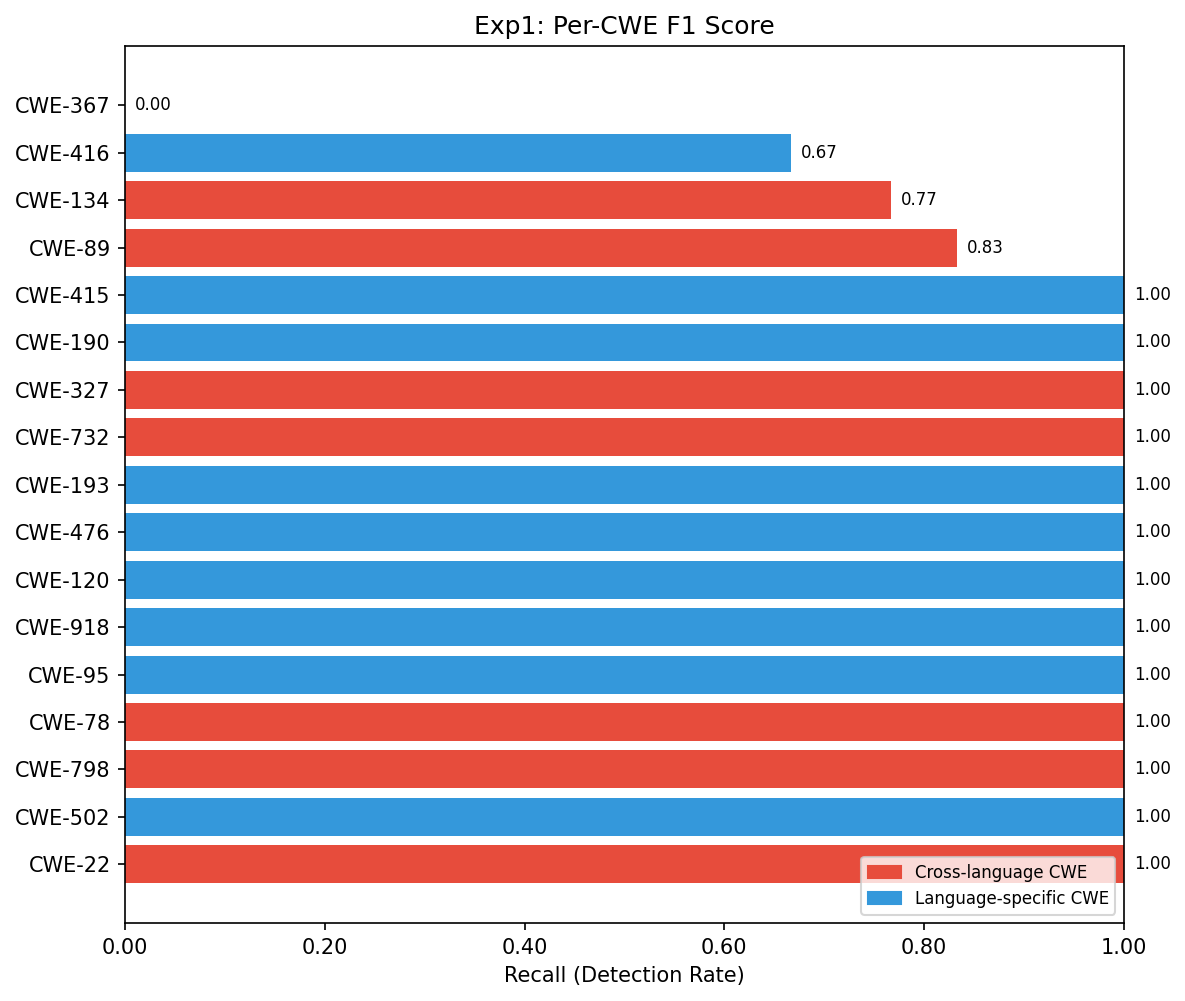
\includegraphics[width=\textwidth]{exp1_per_cwe_f1.png}
    \end{column}
  \end{columns}
  \vspace{0.3em}
  \note{11 of 17 CWE classes reach perfect F1 = 1.00. Hardest: CWE-416 (use-after-free) at 0.667.}
\end{frame}

% =====================================================================
\section{Experiment 2 — Cross-Language Ablation}
% =====================================================================

\begin{frame}{Exp 2: Cross-Language Ablation}
  \begin{center}
    \begin{tabular}{lccc}
      \toprule
      \textbf{Model} & \textbf{Test: C} & \textbf{Test: Python} & \textbf{Test: Joint} \\
      \midrule
      C-only     & 0.861 & 0.811 & 0.836 \\
      Python-only & 0.677 & 0.976 & 0.817 \\
      \textbf{Joint} & \textbf{0.905} & \textbf{0.961} & \textbf{0.931} \\
      \bottomrule
    \end{tabular}
  \end{center}
  \vspace{0.5em}
  \begin{itemize}
    \item Joint training \good{outperforms} single-language training on every test set
    \item C-to-Python transfer (0.811) \good{much better} than Python-to-C (0.677)
    \item Python-only model: precision = 1.00 but recall = 0.596 on C \bad{(recall-biased)}
  \end{itemize}
\end{frame}

\begin{frame}{CWE-Level Transfer: Three Profiles}
  \begin{columns}
    \begin{column}{0.55\textwidth}
      \begin{tabular}{lcc}
        \toprule
        CWE & C-only$\to$Py & Py-only$\to$C \\
        \midrule
        \multicolumn{3}{l}{\textit{Bidirectional}} \\
        CWE-798 (Hardcoded creds) & 1.00 & 1.00 \\
        CWE-22 (Path traversal)   & 1.00 & 0.50 \\
        \midrule
        \multicolumn{3}{l}{\textit{Asymmetric}} \\
        CWE-78 (Cmd injection)    & 1.00 & 0.17 \\
        CWE-89 (SQL injection)    & 0.92 & 0.90 \\
        \midrule
        \multicolumn{3}{l}{\textit{Language-locked}} \\
        CWE-367 (TOCTOU)          & 0.00 & 0.47 \\
        CWE-732 (File perms)      & 1.00 & 0.38 \\
        \bottomrule
      \end{tabular}
    \end{column}
    \begin{column}{0.42\textwidth}
      \begin{block}{Key insight}
        Transfer quality correlates with
        \textbf{surface similarity} of the CWE's
        API across languages ---
        not with semantic similarity of the flaw.
      \end{block}
    \end{column}
  \end{columns}
\end{frame}

% =====================================================================
\section{Training Improvements}
% =====================================================================

\begin{frame}{Failure Modes Found During Development}
  Three failure modes identified on the pre-improvement model:

  \begin{enumerate}
    \item \textbf{CWE-327:} \texttt{hashlib.sha256} (safe) classified as vulnerable at $p = 0.906$
      \begin{itemize}
        \item Model learned \texttt{hashlib} $\to$ vulnerable, not the specific algorithm
      \end{itemize}
    \item \textbf{CWE-78:} \texttt{system()} with a hardcoded path still $p = 0.929$
      \begin{itemize}
        \item No safe \texttt{system()} examples in training
      \end{itemize}
    \item \textbf{Real-world gap:} F1 = 0.410 vs synthetic F1 = 0.931
      \begin{itemize}
        \item Real functions are longer, noisier, more context-dependent
      \end{itemize}
  \end{enumerate}
\end{frame}

\begin{frame}{Intervention 1 — Hard Negative Mining}
  Added 17 safe contrastive examples: \texttt{sha256/sha512} usage, hardcoded \texttt{system()} calls.

  \vspace{0.5em}
  \begin{center}
    \begin{tabular}{llcc}
      \toprule
      CWE & Version & Before & After \\
      \midrule
      CWE-327 & Vulnerable (md5)   & 0.960 & 0.960 \\
      CWE-327 & \good{Fixed (sha256)} & 0.906 & \good{\textbf{0.048}} \\
      CWE-78  & Vulnerable (user input) & 0.958 & 0.959 \\
      CWE-78  & \bad{Fixed (hardcoded path)} & 0.929 & \bad{0.929} \\
      \bottomrule
    \end{tabular}
  \end{center}

  \vspace{0.3em}
  CWE-327 resolved completely. CWE-78 C remains unresolved ---
  distinguishing user-controlled vs hardcoded buffers requires \textbf{data-flow tracking},
  not just surface tokens.
\end{frame}

\begin{frame}{Intervention 2 — Real-World Data Augmentation}
  Added 1{,}000 DiverseVul C/C++ samples to the training set.

  \vspace{0.5em}
  \begin{center}
    \begin{tabular}{lccc}
      \toprule
      Model stage & Synthetic F1 & Real-world F1 & Gap \\
      \midrule
      Synthetic-only (baseline) & 0.931 & 0.410 & $-0.522$ \\
      + Hard negatives          & 0.931 & 0.471 & $-0.460$ \\
      \textbf{+ Real augmentation} & \textbf{0.931} & \textbf{0.749} & $\mathbf{-0.182}$ \\
      \bottomrule
    \end{tabular}
  \end{center}

  \vspace{0.4em}
  \begin{itemize}
    \item Synthetic performance \good{unchanged} throughout
    \item Real-world F1 nearly doubled: $0.410 \to 0.749$
    \item Gap reduced from $-0.522$ to $-0.182$
    \item \textbf{Highest-leverage single intervention in the entire project}
  \end{itemize}
\end{frame}

% =====================================================================
\section{Experiment 3 — Real-World Generalisation}
% =====================================================================

\begin{frame}{Exp 3: Real-World Confusion Matrix}
  \begin{columns}
    \begin{column}{0.45\textwidth}
      \begin{center}
        \begin{tabular}{lcc}
          \toprule
          & \textbf{Pre-aug} & \textbf{Post-aug} \\
          \midrule
          TP  & 66 & \good{88} \\
          FP  & 52 & \good{31} \\
          TN  & 32 & \good{53} \\
          FN  & 50 & \good{28} \\
          \midrule
          FPR & 61.9\% & \good{36.9\%} \\
          FNR & 43.1\% & \good{24.1\%} \\
          \bottomrule
        \end{tabular}
      \end{center}
    \end{column}
    \begin{column}{0.50\textwidth}
      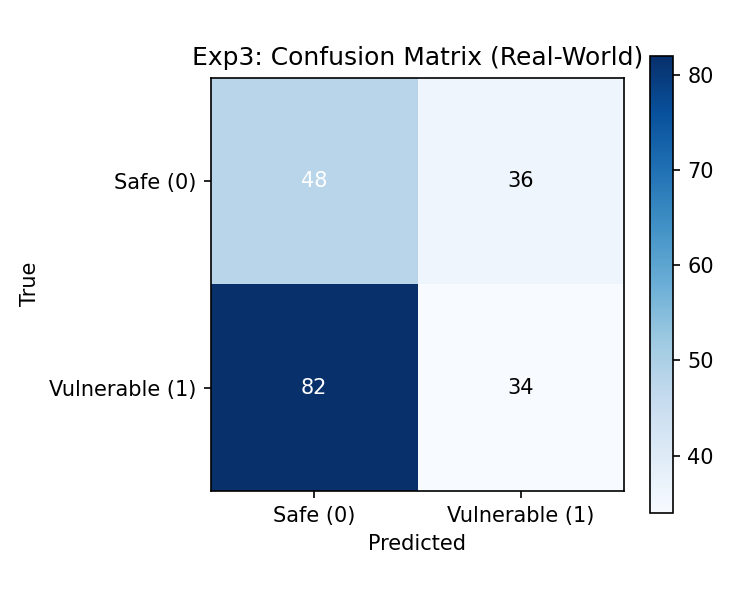
\includegraphics[width=\textwidth]{exp3_confusion_realworld.png}
    \end{column}
  \end{columns}
  \vspace{0.3em}
  Both error rates improve substantially.
  Remaining gap reflects CWE classes \textbf{entirely absent from training}
  (CWE-787, CWE-400, CWE-703).
\end{frame}

% =====================================================================
\section{Semantic Understanding Tests}
% =====================================================================

\begin{frame}{Semantic Understanding Test Suite}
  Four tests distinguish pattern-matching from deeper understanding:

  \vspace{0.5em}
  \begin{center}
    \begin{tabular}{llcc}
      \toprule
      \textbf{Test} & \textbf{What it checks} & \textbf{Passed} & \textbf{Result} \\
      \midrule
      1. Variable renaming  & Robustness to identifier names & 6/6  & \good{Pass} \\
      2. Minimal fix        & Recognising the fixing change   & 7/8  & \good{Near-pass} \\
      3. Dead code          & Control-flow reachability       & 1/5  & \bad{Fail} \\
      4. Token ablation     & No single-token reliance        & 6/6  & \good{Pass} \\
      \midrule
      \textbf{Total}        &                                 & \textbf{20/25} & \\
      \bottomrule
    \end{tabular}
  \end{center}
\end{frame}

\begin{frame}{What the Tests Reveal}
  \begin{columns}
    \begin{column}{0.48\textwidth}
      \textbf{\good{Passing tests confirm:}}
      \begin{itemize}
        \item Representations are not anchored to specific identifier strings
        \item Not triggered by isolated keywords alone
        \item Detects the \emph{structural} change that fixes a vulnerability
          (e.g.\ md5 $\to$ sha256: $p$ drops $0.960 \to 0.048$)
      \end{itemize}
    \end{column}
    \begin{column}{0.48\textwidth}
      \textbf{\bad{Dead code failures reveal:}}
      \begin{itemize}
        \item Code inside \texttt{if(0)} or \texttt{if False:} still triggers a VULNERABLE prediction
        \item Model cannot determine whether a code path is \textbf{reachable}
        \item This requires a control-flow graph --- not available to a sequence encoder
        \item This is an \textbf{architectural ceiling}, not a fixable data problem
      \end{itemize}
    \end{column}
  \end{columns}
\end{frame}

% =====================================================================
\section{Calibration}
% =====================================================================

\begin{frame}{Calibration: Temperature $T = 0.981$}
  \begin{columns}
    \begin{column}{0.50\textwidth}
      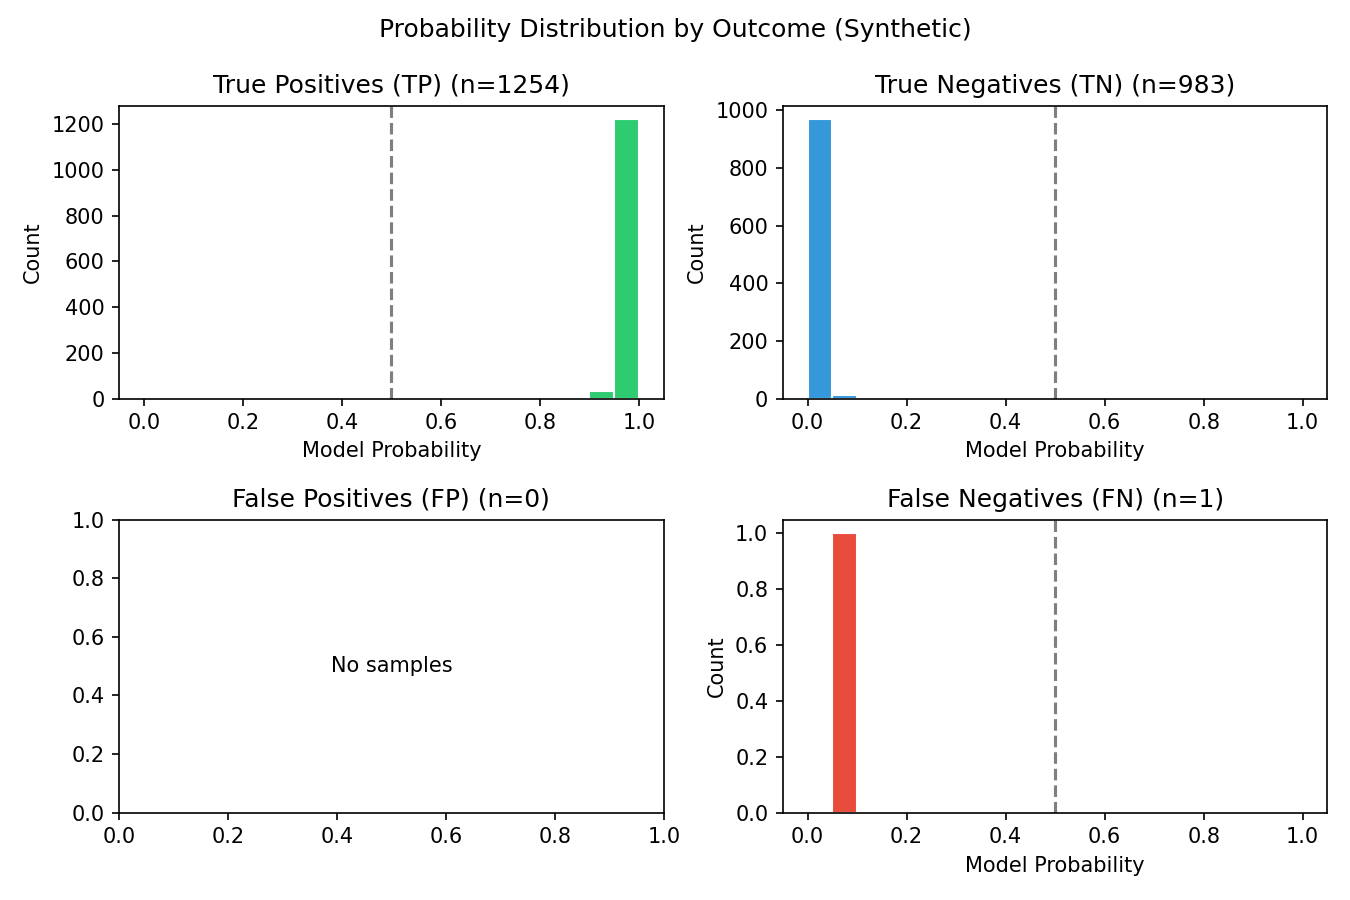
\includegraphics[width=\textwidth]{insight3_calibration_synthetic.png}
    \end{column}
    \begin{column}{0.46\textwidth}
      \begin{itemize}
        \item Temperature scaling: optimal $T = 0.981 \approx 1.0$
        \item Near-unity $T$ means label smoothing already calibrated the model
        \item Synthetic outputs: \textbf{bimodal} --- clearly safe ($p \approx 0$) or clearly vulnerable ($p \approx 0.96$)
        \item Real-world outputs: broader distribution --- more ambiguous partial matches
        \item Outputs can be treated as approximate probabilities for prioritising audit queues
      \end{itemize}
    \end{column}
  \end{columns}
\end{frame}

% =====================================================================
\section{Limitations and Future Work}
% =====================================================================

\begin{frame}{Limitations}
  \begin{enumerate}
    \item \textbf{Architectural} --- Cannot reason about control-flow reachability or data-flow
      provenance. Dead-code and CWE-78 failures follow directly from this.
    \item \textbf{CWE coverage} --- 17 CWE types in training; DiverseVul test set spans $\sim$50.
      Recall on unseen classes is zero.
    \item \textbf{Language coverage} --- C and Python only. Java, JavaScript, Go would require
      additional training data.
    \item \textbf{Synthetic distribution shift} --- Training examples are clean, short, and
      function-isolated. Real code is longer, noisier, and more context-dependent.
    \item \textbf{Real-world evaluation scale} --- 200-sample test set; per-CWE recall
      estimates for low-frequency classes are unreliable.
    \item \textbf{Python real-world data} --- No large Python vulnerability dataset comparable
      to DiverseVul currently exists.
  \end{enumerate}
\end{frame}

\begin{frame}{Future Directions}
  \begin{block}{1. Graph-augmented encoding}
    Add a GNN operating on the data-flow graph to enable taint tracking ---
    directly addressing the CWE-78 data-flow failure.
  \end{block}
  \begin{block}{2. Larger real-world corpus}
    Use more DiverseVul training samples or combine with BigVul.
    The response to real data suggests a 10{,}000-sample augmentation could
    close the remaining gap substantially.
  \end{block}
  \begin{block}{3. CWE class expansion}
    Add synthetic templates for CWE-787, CWE-400, CWE-703 --- the three
    largest false-negative classes in the real-world test.
  \end{block}
  \begin{block}{4. Python real-world evaluation}
    Build a Python vulnerability test set from PyPI/OSV advisories to
    run the same synthetic-to-real analysis for Python.
  \end{block}
\end{frame}

% =====================================================================
\section{Conclusion}
% =====================================================================

\begin{frame}{Summary}
  \begin{center}
    \begin{tabular}{ll}
      \toprule
      \textbf{Contribution} & \textbf{Result} \\
      \midrule
      Multi-language synthetic dataset & 17 CWEs, C + Python, 1{,}230 held-out \\
      Fine-tuned UniXcoder classifier  & F1 = 0.931, AUC = 0.964 (synthetic) \\
      Cross-language ablation (3$\times$3) & Joint $>$ single-language on all sets \\
      Hard negative mining             & sha256 false positive eliminated \\
      Real-world augmentation          & F1: $0.410 \to 0.749$; gap: $-0.522 \to -0.182$ \\
      Semantic understanding suite     & 20/25; ceiling located precisely \\
      \bottomrule
    \end{tabular}
  \end{center}

  \vspace{0.5em}
  \begin{center}
    \textbf{Key takeaway:} A pre-trained code model with careful dataset design,\\
    targeted hard negatives, and real-world augmentation can reach\\
    practically useful multi-language vulnerability detection.\\
    The semantic tests show \emph{what} it has learned --- and \emph{where it stops}.
  \end{center}
\end{frame}

\begin{frame}[plain]
  \begin{center}
    \vspace{2cm}
    {\Large Thank you}\\[1cm]
    {\large Questions?}\\[2cm]
    \note{Code, data, and all experiments available in the dissertation repository.}
  \end{center}
\end{frame}

\end{document}
